\chapter{Herramientas utilizadas}\label{cap.infraestructura}
EL objetivo de este trabajo es preparar la infraestructura para desarrollar prácticas de visión con drones en la plataforma Kibotics\cite{kibotics} tanto con drone real como simulado. Para ello se han necesitado las siguientes herramientas.

\section{Kibotics}
\textit{Kibotics}\cite{kibotics} es una plataforma de enseñanza de robótica infantil desarrollada por las Asociación de robótica JdeRobot\footnote{https://jderobot.github.io}

La batería de ejercicios(figura \ref{fig:kibotics2}) que incluye el entorno \textit{Kibotics}\cite{kibotics} se simula usando el simulador robótico \textit{Websim}. Se trata de un simulador diseñado para el aprendizaje de conceptos básicos de programación de robots especialmente para niños. 
\begin{figure}[H]
  \begin{center}
    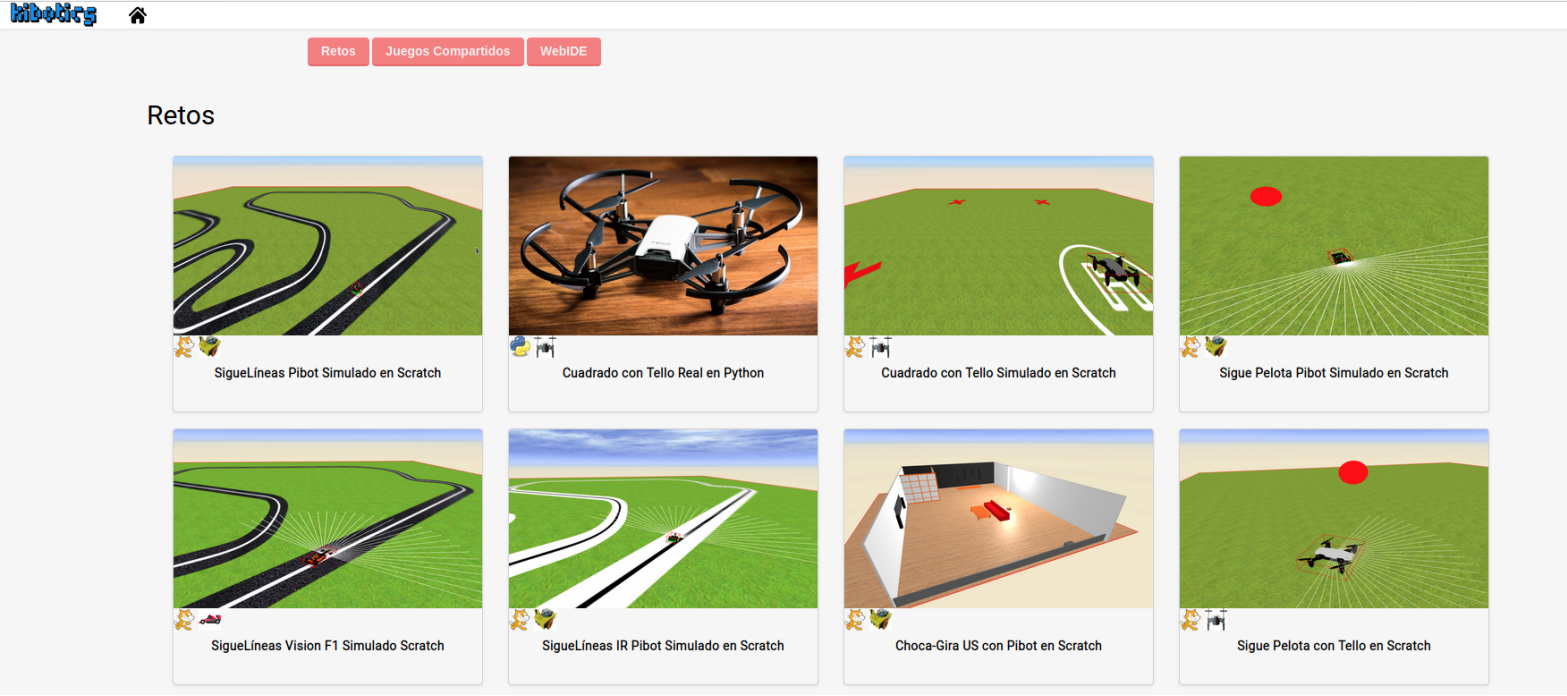
\includegraphics[width=0.6\textwidth]{figures/herramientas/kibotics2.png}
		\caption{Ejercicios Kibotics}
		\label{fig:kibotics2}
		\end{center}
\end{figure}

El simulador permite que los usuarios puedan programar fácilmente los movimientos de los robots, ya que simplemente tienen que acceder a la información que recogen sus sensores y enviar las órdenes precisas a los actuadores del robot. Estas ordenes se deben programar, en \textit{Python} o \textit{Scratch} (figura \ref{fig:kibotics1}), dentro del editor que incorpora la interfaz de \textit{Websim}.
\begin{figure}[H]
  \begin{center}
    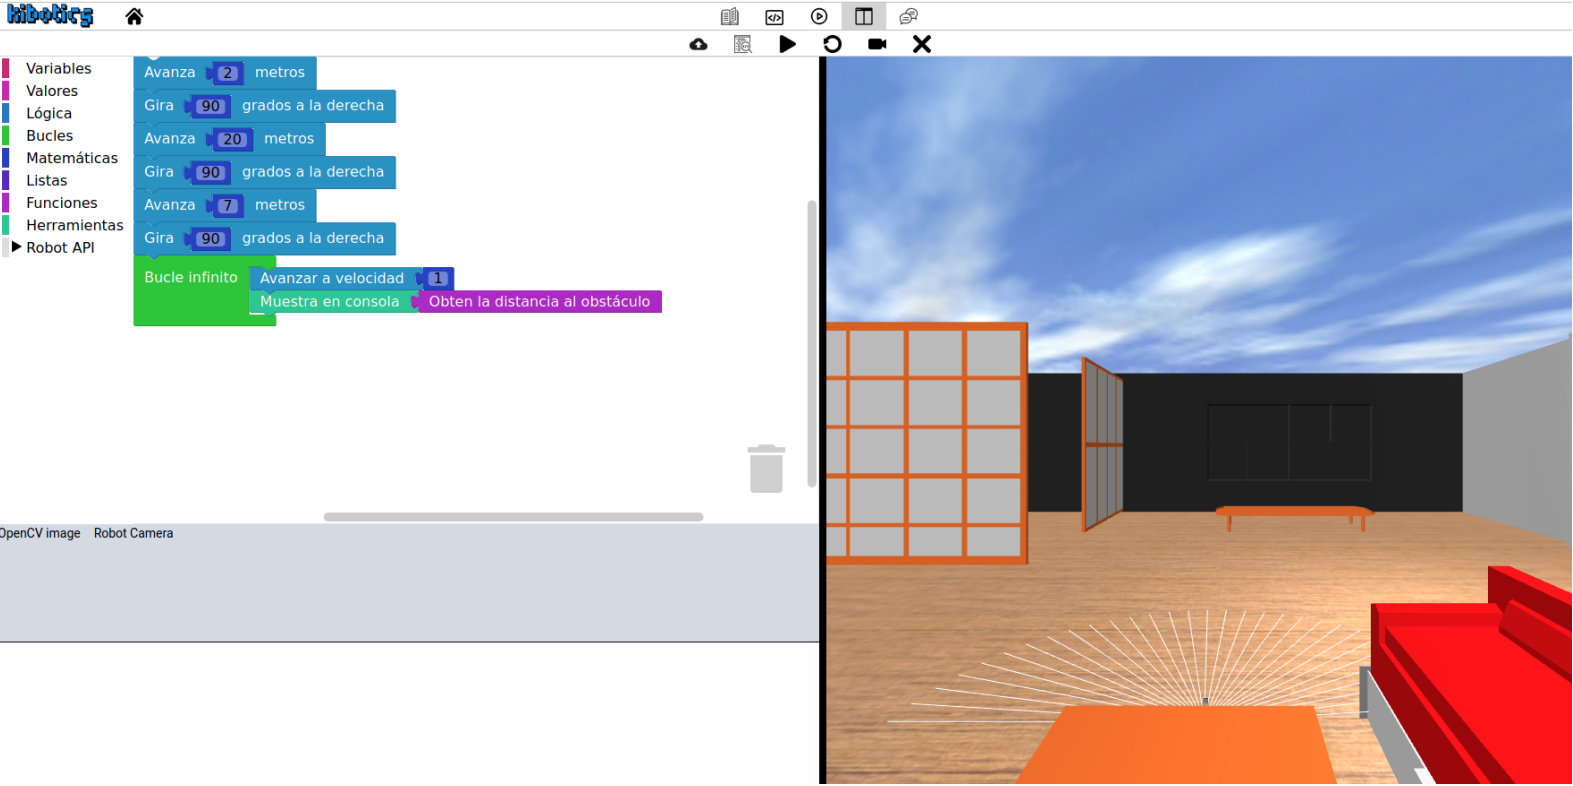
\includegraphics[width=0.6\textwidth]{figures/herramientas/kibotics1.png}
		\caption{Ejercicio con Scratch}
		\label{fig:kibotics1}
		\end{center}
\end{figure}

Se ha usado para la parte simulada.

\section{Tensorflow}
Es una plataforma de código abierto \textit{end-to-end} para el \textit{Machine Learning} que fue liberada bajo licencia de \textit{Apache} 2 a finales de 2015 y que está disponible en github~\cite{github_tensorflow}. Fue desarrollada por el equipo de investigación en \textit{Machine Learning “Google Brain”}  en \textit{C++} y \textit{Python} y es usada en multitud de productos y servicios de Google como Gmail o \textit{Google Translation}. Google ofrece en su plataforma \textit{Cloud} ejecutar \textit{Tensorflow} en \textit{Tensor Processing Unit} (TPU), un nuevo tipo de procesadores en \textit{Cloud} optimizados para ejecutar \acrfull{ia}.  \textit{TensorFlow} está orientado a problemas de \textit{Deep Learning} y permite entrenar y construir redes neuronales. 

\textit{TensorFlow} puede correr tanto en CPUs como en GPUs (haciendo uso de \textit{\acrfull{cuda}}). Está disponible en \textit{Linux} de 64 bits, \textit{MacOS}, y plataformas móviles que incluyen \textit{Android} e \textit{iOS}, además ha incluido soporte para \textit{Javascript}, por lo que puede ser usado en cualquier navegador. Actualmente es el entorno más popular en \textit{Deep Learning}.

Puede ejecutar de forma rápida y eficiente gráficos de flujo. Un gráfico de flujo está formado por operaciones matemáticas representadas sobre nodos, y cuya entrada y salida es un vector multidimensional o tensor de datos, por este motivo recibe el nombre de \textit{TensorFlow}.

Las ventajas de este software se extienden a muchas disciplinas a parte de la tecnología TIC. Se emplea en imágenes médicas para la detección de tumores por ejemplo, también se usa en la detección y combinación de estilos artísticos en la pintura, etc.

En este \acrshort{tfm} se emplean la versión 1.15.0 y 2.2.0 de \textit{Tensorflow} para \textit{Python} y la versión 2.0.1 para \textit{Javascript}.
\subsection{Object Detection API}
\textit{Object Detection \acrshort{api}} \footnote{\url{https://github.com/tensorflow/models/tree/master/research/object_detection}} es un \textit{framework} de código abierto construido sobre \textit{TensorFlow} que facilita la construcción, el entrenamiento y el despliegue de modelos de detección de objetos desarrollado por \textit{Google}. Todas las redes de detección preentrenadas que se pueden descargar desde la web de \textit{Tensorflow} han sido entrenadas con este \acrshort{api}.

Hasta Julio de 2020, cuando publicaron la primera versión con soporte para \textit{Tensorflow} 2.x, solo tenía solo soporte para la versión 1.x.

\section{Opencv}
\textit{OpenCV} \footnote{https://opencv.org/} es una librería de código abierto desarrollada por \textit{Intel} y publicada  bajo licenciade BSD. Esta librería implementa gran variedad de herramientas para la interpretación de la imagen. Sus  siglas  provienen  de  los  términos anglosajones ``\textit{Open Source Computer  Vision Library}", y tal y como se puede deducir es una librería destinada a aplicaciones de visión por computador en tiempo real. Puede ser empleada en MacOS, Windows y Linux, y existen versiones para \textit{C\#}, \textit{Python} y \textit{Java}, a pesar de que originalmente era una librería en \textit{C/C++}. Además hay interfaces para \textit{Ruby}, \textit{Python}, \textit{Matlab} y otros lenguajes.

En 2017 añadieron \textbf{soporte para \textit{Javascript}} mediante \textit{emscripten}\footnote{https://emscripten.org} que es un software que permite convertir bibliotecas escritas en \textit{C++} en binarios para \textit{Javascript}. Esto permite tener muchas de las funcionalidades desarrolladas en \textit{C++} en el navegador.

\textit{OpenCV} implementa algoritmos para técnicas de calibración, detección de rasgos, rastreo, análisis de la forma, análisis del movimiento, reconstrucción 3D, segmentación de objetos y reconocimiento, etc. Los algoritmos se basan  en  estructuras de datos flexibles acopladas con estructuras IPL (\textit{Intel  Image Processing Library}), aprovechándose de la arquitectura de Intel en la optimización de más de la mitad de las funciones. Incorpora funciones básicas para modelar el fondo, sustraer dicho  fondo y generar imágenes de movimiento MHI  (\textit{Motion  History  Images}).  Además  incluye  funciones para determinar dónde hubo movimiento y en qué dirección. 

\begin{figure}[H]
  \begin{center}
    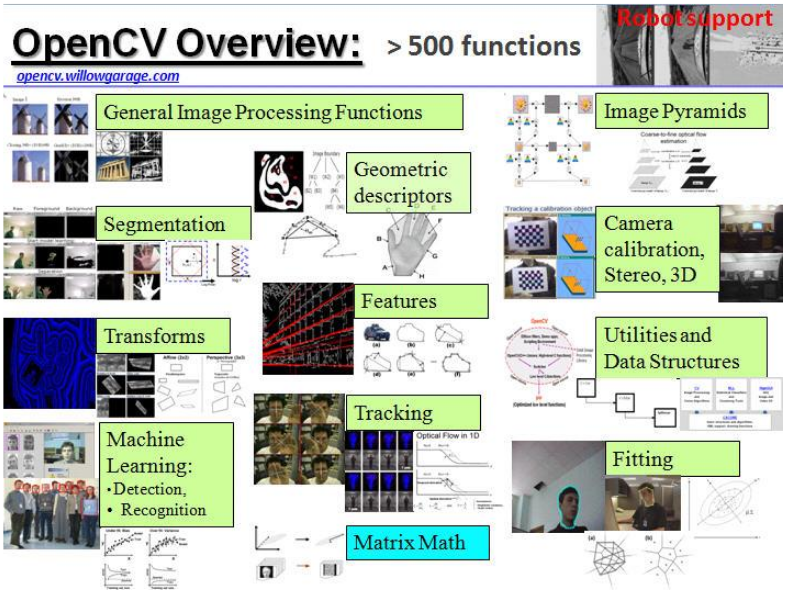
\includegraphics[width=0.6\textwidth]{figures/herramientas/opencv.png}
		\caption{Funciones de OpenCV}
		\label{fig.opencv}
		\end{center}
\end{figure}

Fue diseñado para tener una alta eficiencia computacional, está escrito en C y puede aprovechar las ventajas de los procesadores multinúcleo. Contiene más  de  2500  funciones  que  abarcan  muchas  áreas  de  la  visión  artificial.  También  tiene  una librería   de   aprendizaje   automático   (MLL,  \textit{Machine   Learning   Library})   destinada   al reconocimiento  y agrupación de patrones estadísticos.

Desde su aparición \textit{OpenCV} ha sido usado en numerosas aplicaciones. Entre las cuales se encuentra la unión de imágenes de satélites y mapas web, la reducción de ruido en imágenes  médicas,  los  sistemas  de  detección  de movimiento,  la  calibración  de  cámaras,  el manejo  de  vehículos  no  tripulados, el  reconocimiento  de  gestos, etc. \textit{OpenCV} es empleado también en reconocimiento de música y sonido, mediante la aplicación de técnicas de reconocimiento de visión en imágenes de espectrogramas del sonido.

Hay  una  gran  cantidad  de  empresas    y  centros  de  investigación  que  emplean  estas técnicas como IBM, Microsoft, Intel, SONY, Siemens, Google, Stanford, MIT, CMU, Cambridge e INRIA.

En este proyecto se hace uso de la versión \textit{OpenCV} 4.2 de \textit{Python} y 3.3.1 de \textit{Javascript}.
\section{Google Colaboratory}
\textit{Google Colaboratory o colab}\footnote{\url{https://colab.research.google.com}} (figura \ref{fig:colab})  es un servicio de \textit{Google} que permite ejecutar código \textit{Python} desde el navegador basándose en la tecnología \textit{Jupyter notebook}\footnote{\url{https://jupyter.org}}. En el servidor hay un interprete de \textit{Python} que recibe el código que se escribe en el navegador y devuelve el resultado para mostrarlo en su celda correspondiente.

La mayor ventaja de este servicio con respecto a ejecutar el propio código en local es que se tiene acceso tanto a \textit{GPUs} como a \textit{TPUs} proporcionadas por \textit{Google}, es decir, se pueden hacer cálculos muy costosos computacionalmente en ordenadores básicos.

\begin{figure}[H]
  \begin{center}
    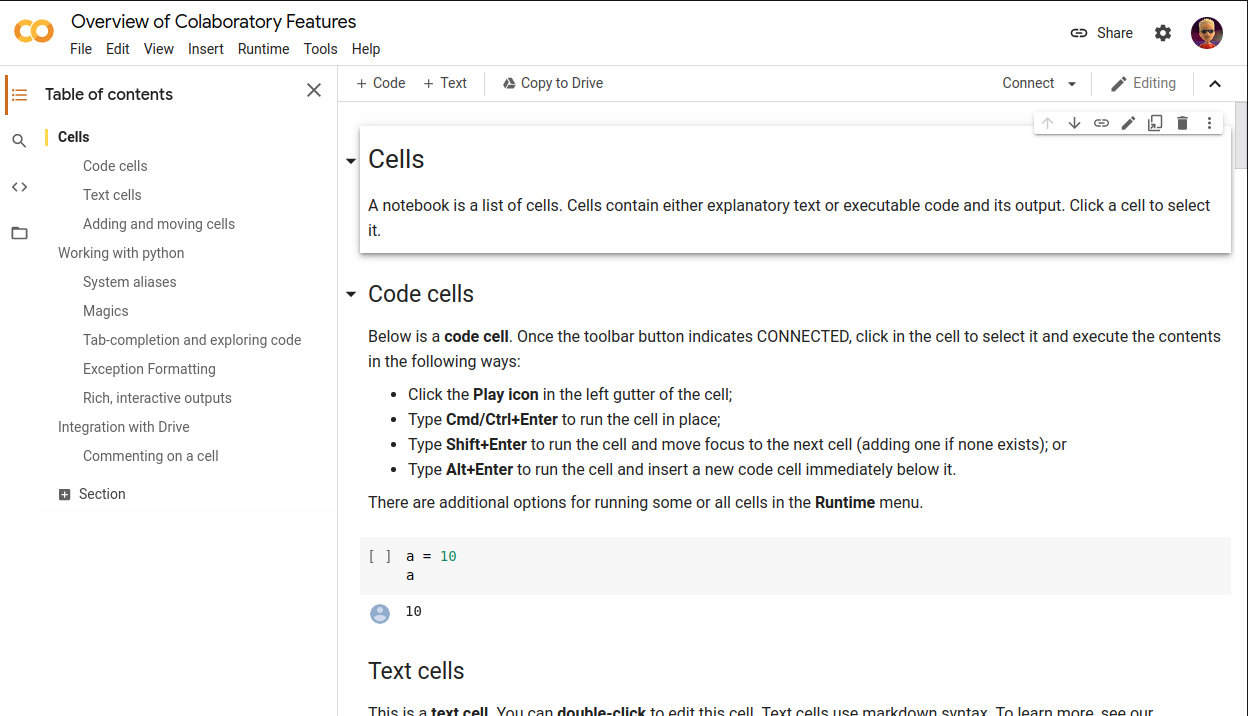
\includegraphics[width=0.6\textwidth]{figures/herramientas/colab.png}
		\caption{Google colab}
		\label{fig:colab}
		\end{center}
\end{figure}
\section{DJI Tello}
Es un pequeño drone (figura \ref{fig:tello}) fabricado por la empresa DJI \footnote{\url{https://www.dji.com/es}}. Tiene las ventajas de ser programable mediante un \acrshort{api} además de tener un precio muy razonable, en torno a 100€, lo que le permite ser una muy buena opción de cara a la enseñanza.
\begin{figure}[H]
  \begin{center}
    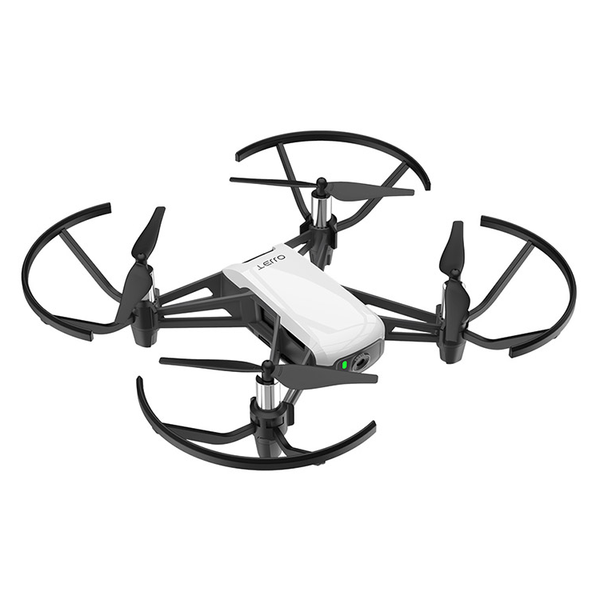
\includegraphics[width=0.4\textwidth]{figures/herramientas/tello.png}
		\caption{Drone Tello}
		\label{fig:tello}
		\end{center}
\end{figure}
\section{Mixamo}
\textit{Mixamo}\cite{mixamo} es una empresa del grupo \textit{Adobe Systems} que desarrolla y vende servicios basados en la web para la animación de personajes en 3D. Utilizan métodos de \textit{Machine Learning} para automatizar los pasos del proceso de animación de personajes, incluyendo desde el modelado 3D hasta la animación 3D. Desde su web ofrecen modelos y animaciones gratuitos (\ref{fig.mixamo}).
\begin{figure}[H]
  \begin{center}
    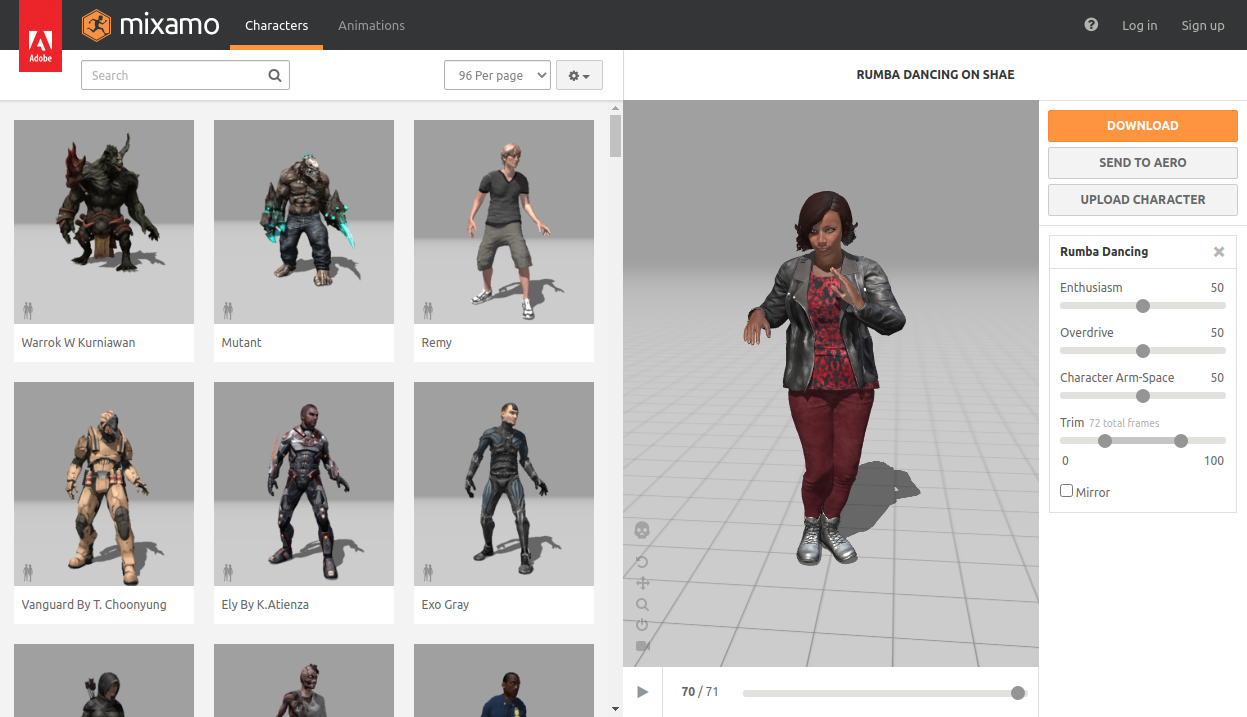
\includegraphics[width=0.6\textwidth]{figures/herramientas/mixamo.png}
		\caption{Ejemplos de Mixamo}
		\label{fig.mixamo}
		\end{center}
\end{figure}
En este proyecto se ha usado para obtener los modelos de las personas para la versión simulada.
\section{Blender}
\textit{Blender}\footnote{\url{https://www.blender.org}} (figura \ref{fig:blender}) es un programa dedicado especialmente al modelado, iluminación, renderizado, animación y creación de gráficos tridimensionales.

Inicialmente fue distribuido de forma gratuita pero sin el código fuente. Posteriormente pasó a ser software libre. Actualmente es compatible con todas las versiones de Windows, macOS, GNU/Linux (incluyendo Android), Solaris, FreeBSD e IRIX.
\begin{figure}[H]
  \begin{center}
    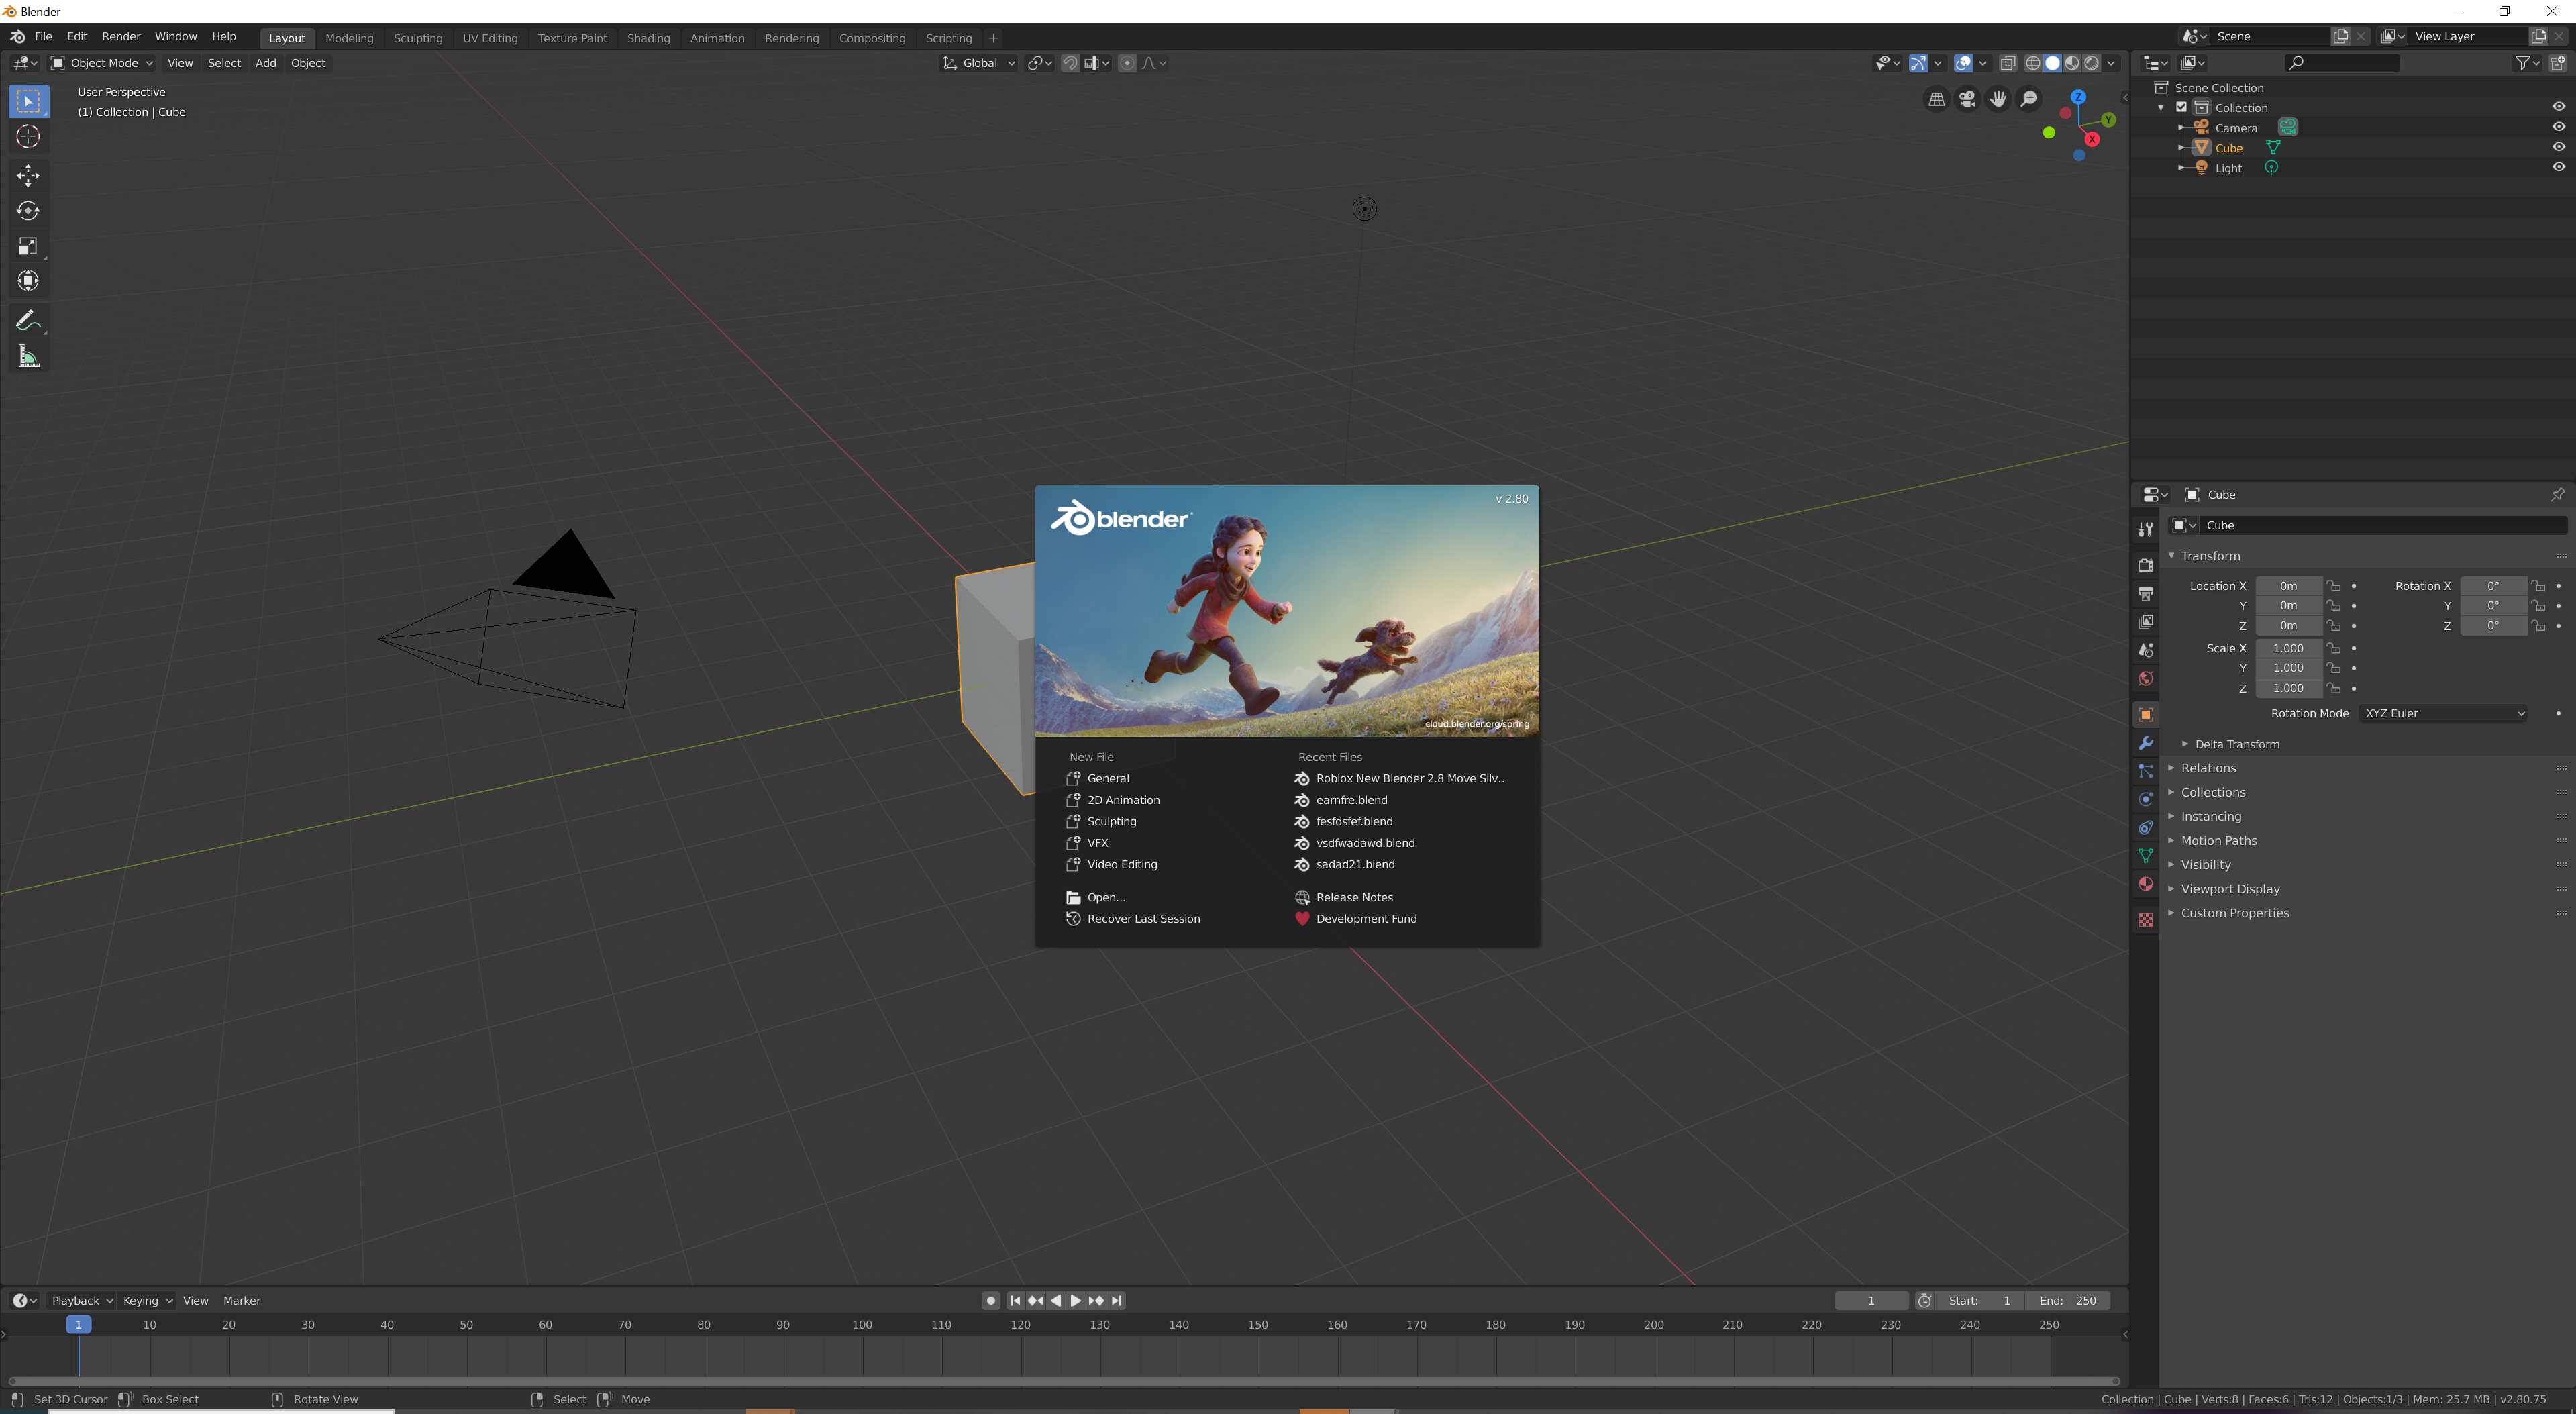
\includegraphics[width=0.6\textwidth]{figures/herramientas/blender.png}
		\caption{Blender}
		\label{fig:blender}
		\end{center}
\end{figure}
En este \acrshort{tfm} se ha usado para modificar los modelos extraídos de \textit{Mixamo}
\section{LabelMe}
\textit{LabelMe}\cite{labelme} es un proyecto creado por el Laboratorio de Ciencias de la Computación e Inteligencia Artificial del MIT (CSAIL) que proporciona un conjunto de datos de imágenes digitales con anotaciones. Además también tiene una herramienta de etiquetado\ref{fig:labelme} de \textit{datasets} que permite subir tu propio \textit{dataset} a un servidor para poder etiquetar cada imagen desde el navegador.
\begin{figure}[H]
  \begin{center}
    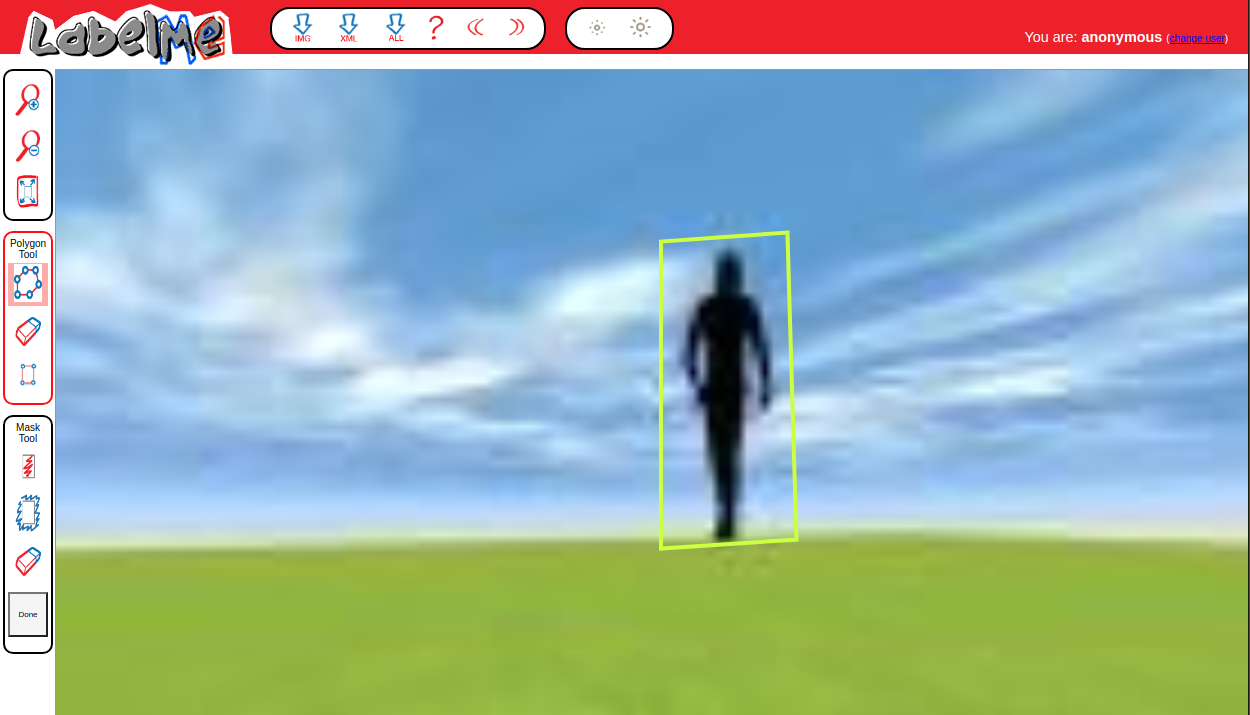
\includegraphics[width=0.6\textwidth]{figures/herramientas/labelme.png}
		\caption{Etiquetado de LabelMe}
		\label{fig:labelme}
		\end{center}
\end{figure}

En este proyecto se ha usado etiquetar el \textit{dataset} para el reentrenamiento de la red para el simulador.
